\begin{figure}[!htb]
  \centering
  \begin{subfigure}[b]{0.3\textwidth}
    \centering
    
\includegraphics[width=\textwidth,scale=0.5]{Chapter5/figures/3pb/beta_0.1_e0_0.8}
    \caption{$\varepsilon_0=0.8$}
  \end{subfigure}
  \begin{subfigure}[b]{0.3\textwidth}
    \centering
    
\includegraphics[width=\textwidth,scale=0.5]{Chapter5/figures/3pb/beta_0.1_e0_0.4}
    \caption{$\varepsilon_0=0.4$}
  \end{subfigure}
  \begin{subfigure}[b]{0.3\textwidth}
    \centering
    
\includegraphics[width=\textwidth,scale=0.5]{Chapter5/figures/3pb/beta_0.1_e0_0.2}
    \caption{$\varepsilon_0=0.2$}
  \end{subfigure}
  
  \begin{subfigure}[b]{0.3\textwidth}
    \centering
    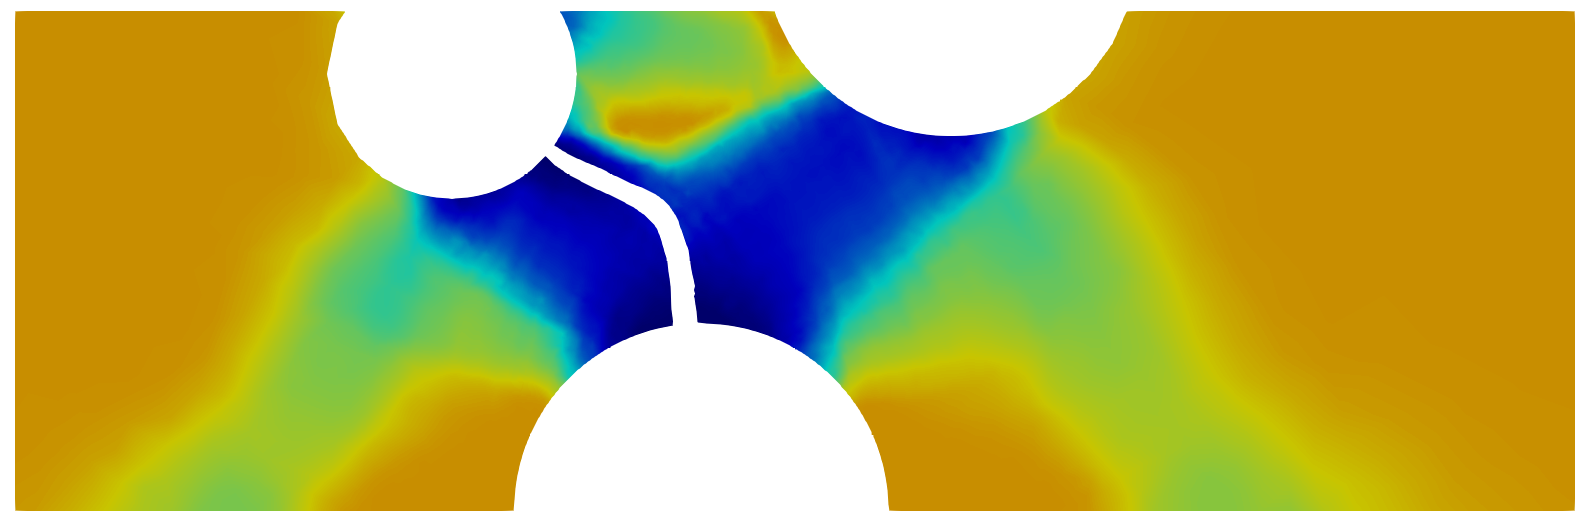
\includegraphics[width=\textwidth,scale=0.5]{Chapter5/figures/3pb/beta_0.1_e0_0.1}
    \caption{$\varepsilon_0=0.1$}
  \end{subfigure}
  \begin{subfigure}[b]{0.3\textwidth}
    \centering
    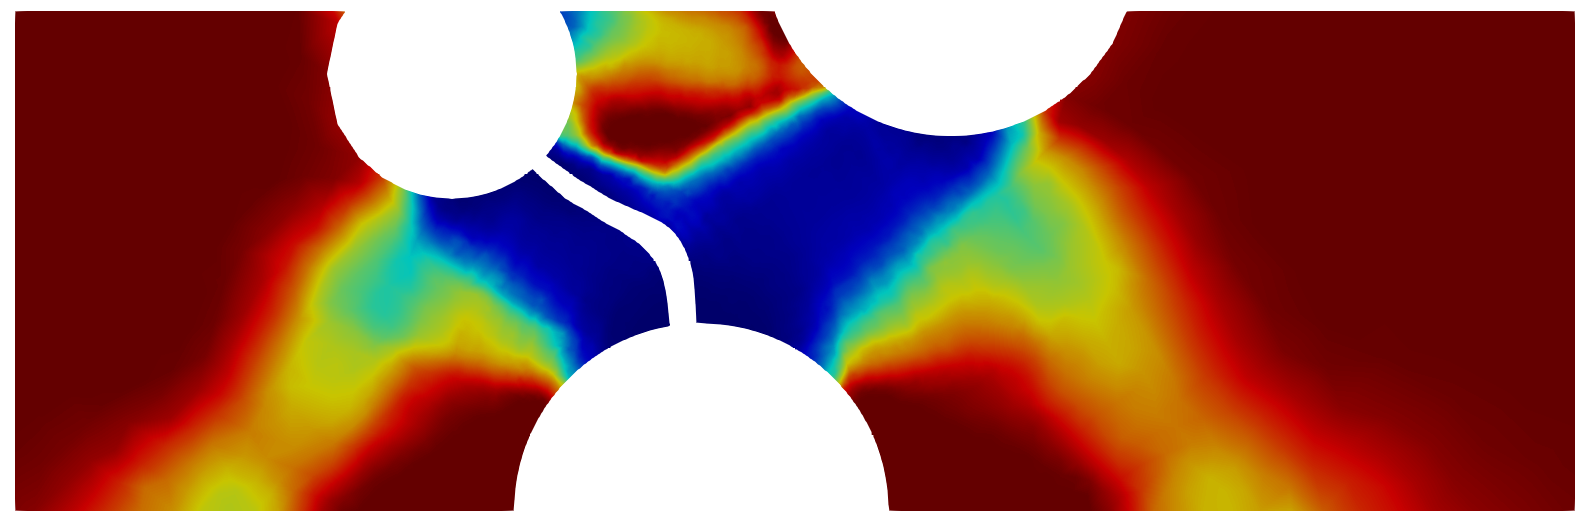
\includegraphics[width=\textwidth,scale=0.5]{Chapter5/figures/3pb/beta_0.1_e0_0.05}
    \caption{$\varepsilon_0=0.05$}
  \end{subfigure}
  \begin{subfigure}[b]{0.3\textwidth}
    \centering
    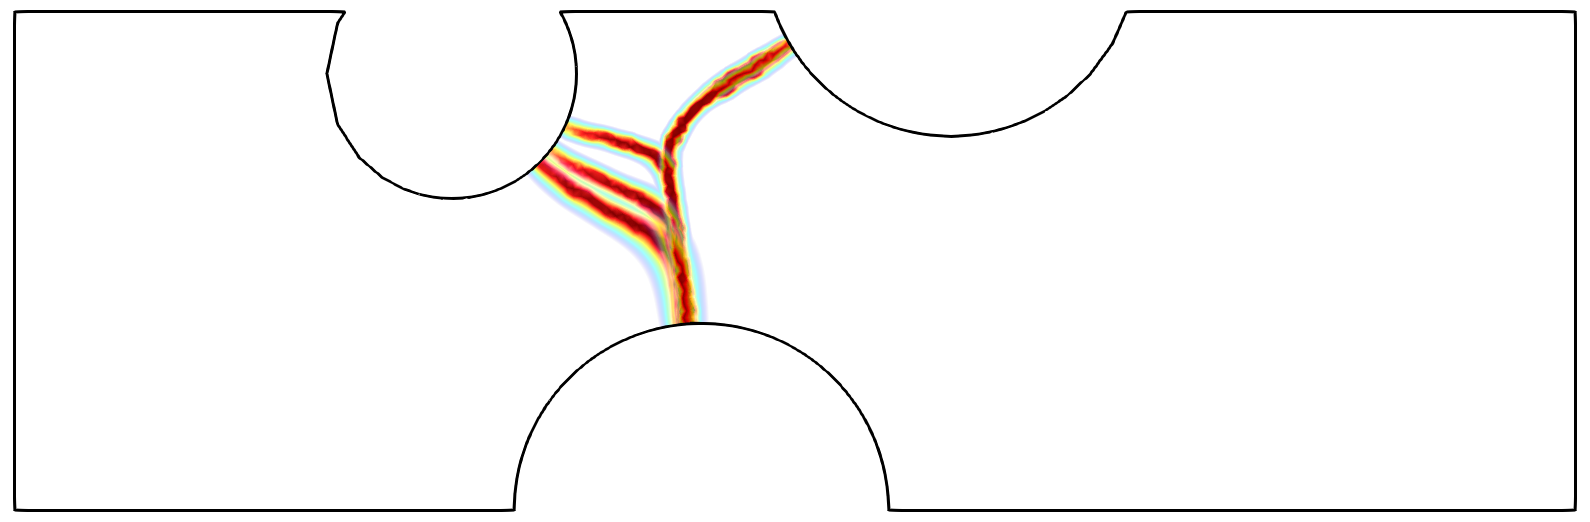
\includegraphics[width=\textwidth,scale=0.5]{Chapter5/figures/3pb/compare_beta_constant}
    \caption{}
  \end{subfigure}
  \caption{(a-e) Contour plots of the effective fracture toughness $\widehat{\Gc}$ with $\beta=0.1$ and different values of $\varepsilon_0$, using the E-P-D model. The portion of the domain with $d > 0.8$ is removed to visualize the crack path. (f) Superposition of the damage contours. All contours are plotted on the reference configuration for the purpose of comparison.}
  \label{fig: Chapter5/3pb/2D_comparison_constant_beta}
\end{figure}
